\documentclass[12pt]{article}
\title{Case Study}
\usepackage{amsmath} %dfrac
\usepackage{graphicx}

\begin{document}

\section{Methodology}

To characterize the behavior and estimate the benefit of the approach
proposed in this paper, a case study of representative tasks was
performed. The tasks were selected from Malardalen University of
Sweden's WCET benchmark suite[1]. Each task was built using Gaisler's
Bare-C Cross Compiler[2] for the GRSIM LEON3[3] simulated target. 

After compiling and linking, each task was analyzed by AbsInt's
a\textsuperscript{3} WCET[4] tool. This yielded the basic block
boundaries within each task. Next, the basic blocks
${\{B_1, B_2, ..., B_n\}}$ were serialized based upon an understanding of
the control flow of the task. Program points
${\{P_1, P_2, ..., P_n\}}$ were assigned by setting ${P_i}$ to the
address of the final instruction of each basic block ${B_i}$ for ${i}$
from ${0}$ to ${n}$.

Each program point ${P_j}$ served as a breakpoint within the task when
running on the simulator. The task was executed, recording the state of
the instruction ${C^I_j}$ and data ${C^D_j}$ cache state for every
visit of ${P_j}$. Given the limitations of the simulator and
a\textsuperscript{3} it was not possible record the actual control
flow. Thus, definitively over-estimating the UCBs shared between two
program points was not possible.

Instead, all instruction and data cache state was disregarded except
the state collected during the final visit of ${P_j}$ during the tasks
execution. Using these final snapshots the UCBs shared between two
program points ${P_i}$ and ${P_j}$ are determined by the following
equation.

\begin{center}
  ${\bigcap_{k=i}^{j-1} C_k}$
\end{center}

This intersection of the cache state taken from program point ${P_i}$
to the penultimate point ${P_{j-1}}$ serves as an upper bound on the
actual UCBs shared between the two points ${P_i}$ and ${P_j}$. Since
the UCBs are the primary factor of CRPD, the results are presented in
terms of UCB counts.

\subsection{Availability}

This method may be verified and reproduced using the same tools and
data. Gaisler's compiler and simulator are freely available. AbsInt's
a\textsuperscript{3} tool is available for educational and evaluation
purposes. The programs written and data used in this paper can be
found on GitHub at the following url:

\begin{center}
https://github.com/ctessler/superblocks/tree/master/study
\end{center}


\section{Results}

The results are presented as a comparison between the method described
herein and the Bertonga approach. For a program point ${P_j}$ the
Bertogna approach defines the UCBs (and therefor the CRPD) as:

\begin{equation*}
  max\{ UCB(P_i, P_j) \vert i < j \}
\end{equation*}

To determine the maximum benefit of the new approach, the best case
scenario is considered. When the preemption point is selected with the
fewest number of UCBs based upon previous preemption.  For ${P_j}$ the
determination is made by:

\begin{equation*}
  min\{ UCB(P_i, P_j) \vert i < j \}
\end{equation*}

In the following graph, the x-axis is a program point ${P_i}$. The
y-axis is the number of UCBs shared with a later program point. For
the red line, the later point is the one with the maximum number of
shared UCBs. For the green line, the later point is the one with the
minimum number of UCBs.

Bertogna's approach is represented by the red line. The proposed
approach by the green line. For both approaches only two points are
considered for possible preemption. Bertogna's approach would select
the two points related to the lowest y-value of the red line. The
proposed approach would select the lowest y-value of the green line.

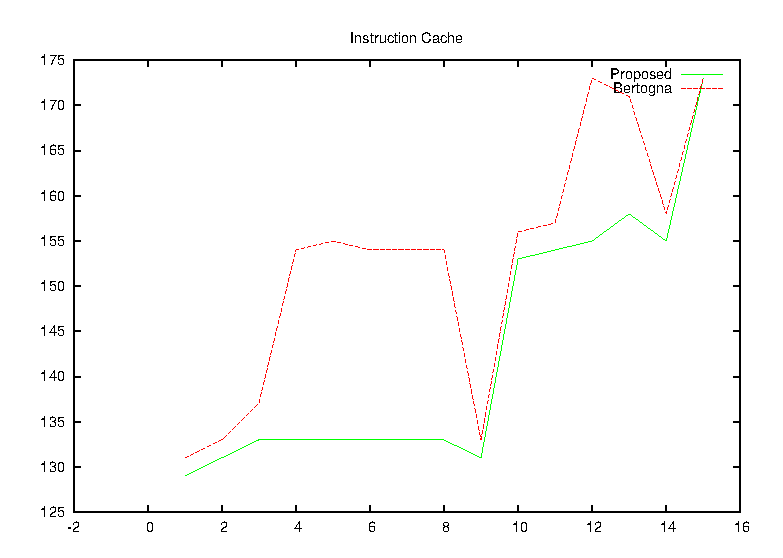
\includegraphics{eps/bsort-icache.eps}

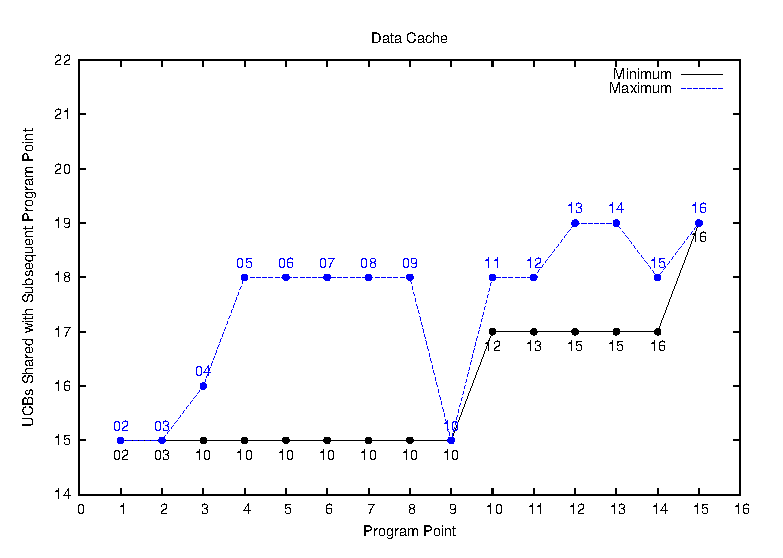
\includegraphics{eps/bsort-dcache.eps}

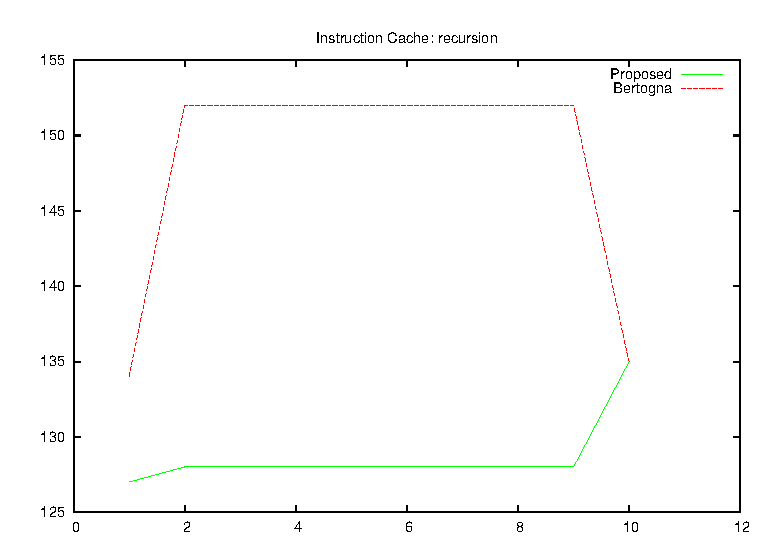
\includegraphics{eps/recursion-icache.eps}

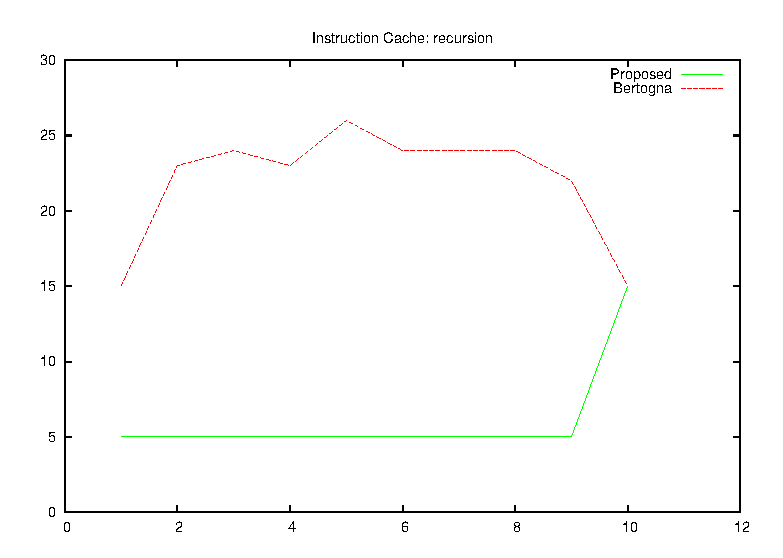
\includegraphics{eps/recursion-dcache.eps}

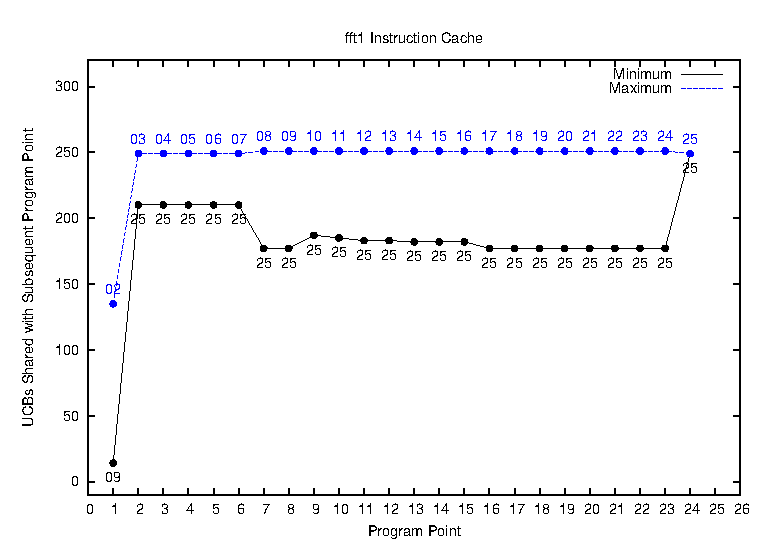
\includegraphics{eps/fft1-icache.eps}

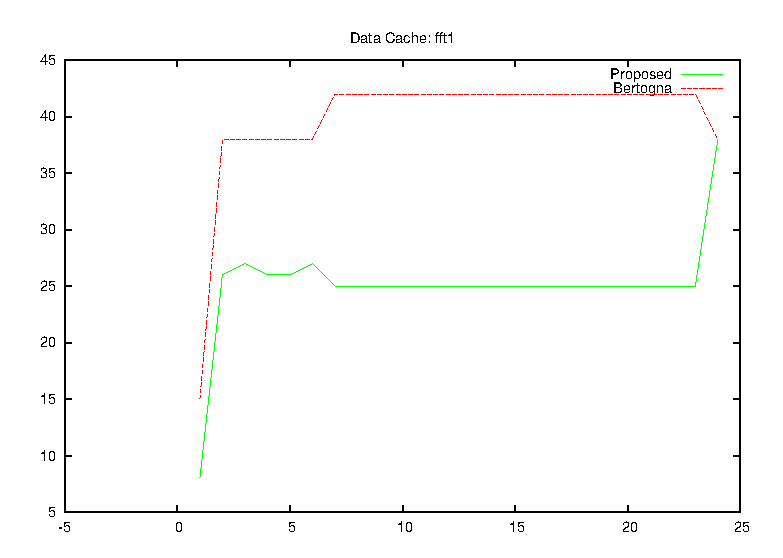
\includegraphics{eps/fft1-dcache.eps}

For the bsort task, the overall benefit for instruction and data
caches is 2 and 0 UCBs. For the fft1 task, the instruction and data
cache benefit is 121 and 7 UCBs. For the recursion task, the benefit
is 7 and 10 UCBs.

\section{References}

\begin{enumerate}
\item MRTC Benchmarks \\
http://www.mrtc.mdh.se/projects/wcet/benchmarks.html

\item Gaisler Compiler  \\
http://gaisler.com/index.php/downloads/compilers

\item Gaisler GRSIM \\
http://gaisler.com/index.php/products/simulators/grsim

\item AbsInt a\textsuperscript{3} WCET Tool \\
http://www.absint.com/a3/index.htm
\end{enumerate}


\end{document}

